\chapter{基于多编码器混合自注意网络的医学视觉问答研究}
本章提出一种多编码器混合自注意网络(Multi-Encoder Mixture Self-Attention Network,MEMSA)用其展开对医学视觉问答(MED-VQA)问题的研究,在传统采用单一自编码器进行图像编码的模型中分别加入元学习,对比学习等方法训练混合编码器模型
,多个编码器可以从不同的"视角"和维度,充分挖掘并提取图像信息,获得更丰富的信息表征能力,是一种有效的视觉增强方法\cite{nguyen2019overcoming}。同时采用跨模态自注意力的思想融合不同模态的编码信息,以获得模态间重要的特征关联。
实验证明,多编码器混合方法以及自注意网络都有效地提高了MED-VQA模型在特征提取部分的融合表征能力,从而提高了视觉问答模型的问答准确率。

\section{多编码器混合自注意网络}
\subsection{MEMSA网络架构}
在计算机科学领域,每个问题往往都有着一套通用的解决方案和基础结构。目前解决VQA问题的模型基本方法是Q(问题)+I(图像)的联合嵌入方法\cite{malinowski2015ask}。
该方法的框架如图\ref{Framwork}所示,由主要由特征提取、特征融合、回答预测三部分构成,包含图像编码器、文本编码器、特征融合算法模型以及根据任务
需要设计的回答预测四大组件。

\subsubsection*{MEMSA网络架构}
\begin{figure}[htbp]
	% 图片居中(列居中对齐)
	\centering	
	% 包含当前路径下的Fig文件夹的图片文件
	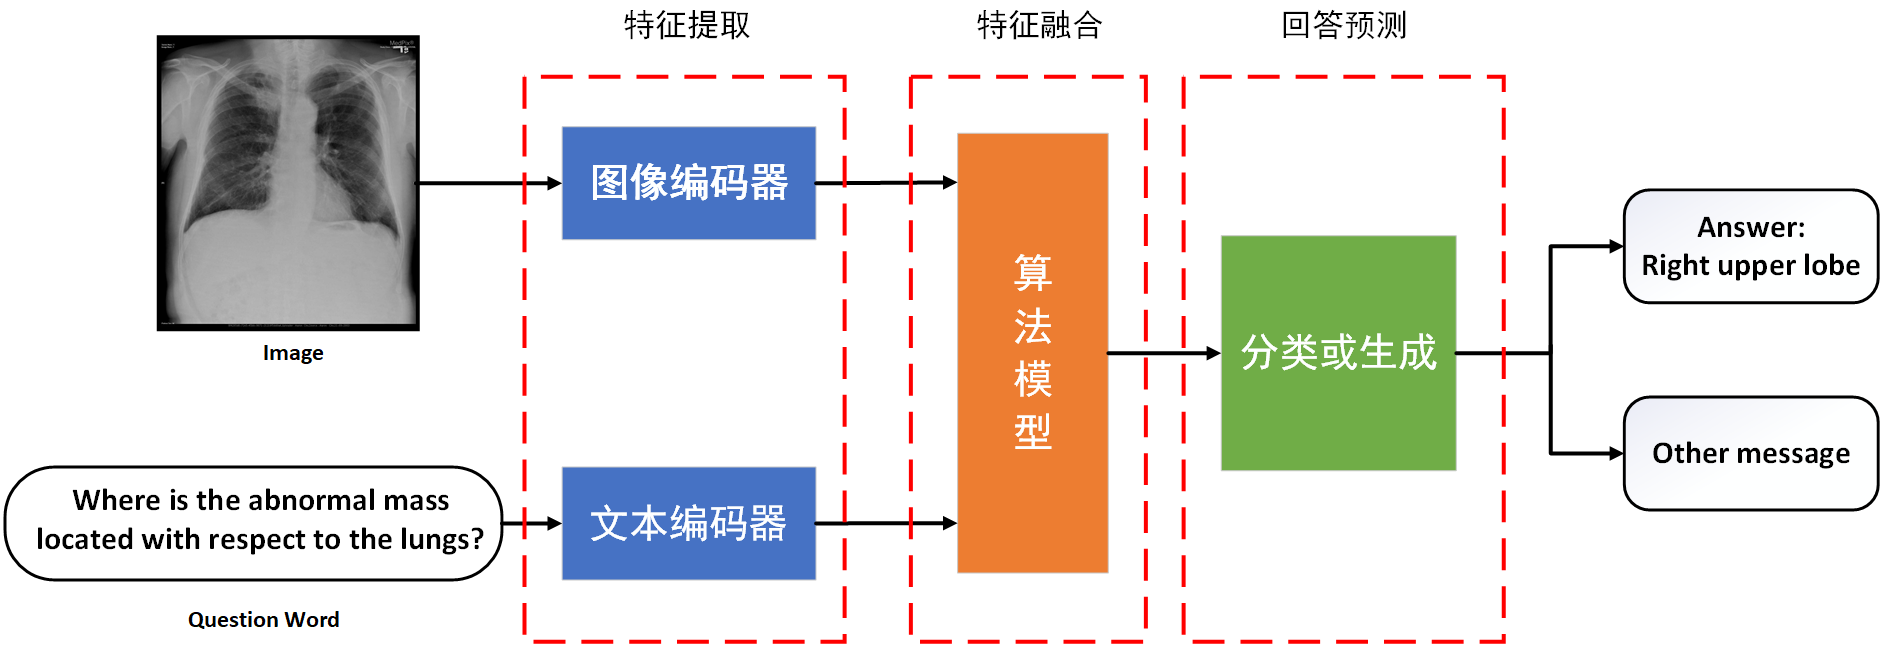
\includegraphics[width=1\textwidth]{Fig/myfig/chapter3/popline2.png}  %scale = 0.3
	% 添加标签one_DFUAV以及图标题“XXX”,引用某图时使用\ref{xxx},其中xxx就是标签,图编号是自动生成的。
	\caption{\label{Framwork}总体框架} 
\end{figure}
如图\ref{Framwork},Med-VQA中图像编码器使用的一般是目前比较成熟的卷积神经网络,如VGGNet、ResNet;文本编码器主要用于编码问题句子,常用的有目前主流的语言编码模型,如LSTM、Bert等。
编码器通常都使用预训练权重进行初始化,在训练过程中可以冻结也可以用端到端的方式进行微调。特征融合以及算法部分目前主流的方式有加权融合,拼接融合,注意力融合等方法。
回答预测部分根据任务的不同往往采用不同的设计:如针对分类问题,组件通常是一个神经网络分类器;针对生成问题,组件通常是循环神经网络(RNN)语言生成器或者注意力模型。

\subsubsection*{MEMSA模型设计}
依据上述视觉问答的基本框架,并针对当前医学视觉问答(Med-VQA)问题存在的几大难点提出了如图\ref{fig:memsa}所示的多编码器混合自注意网络模型(MEMSA):
\begin{figure}[htbp]
	% 图片居中(列居中对齐)
	\centering	
	% 包含当前路径下的Fig文件夹的图片文件
	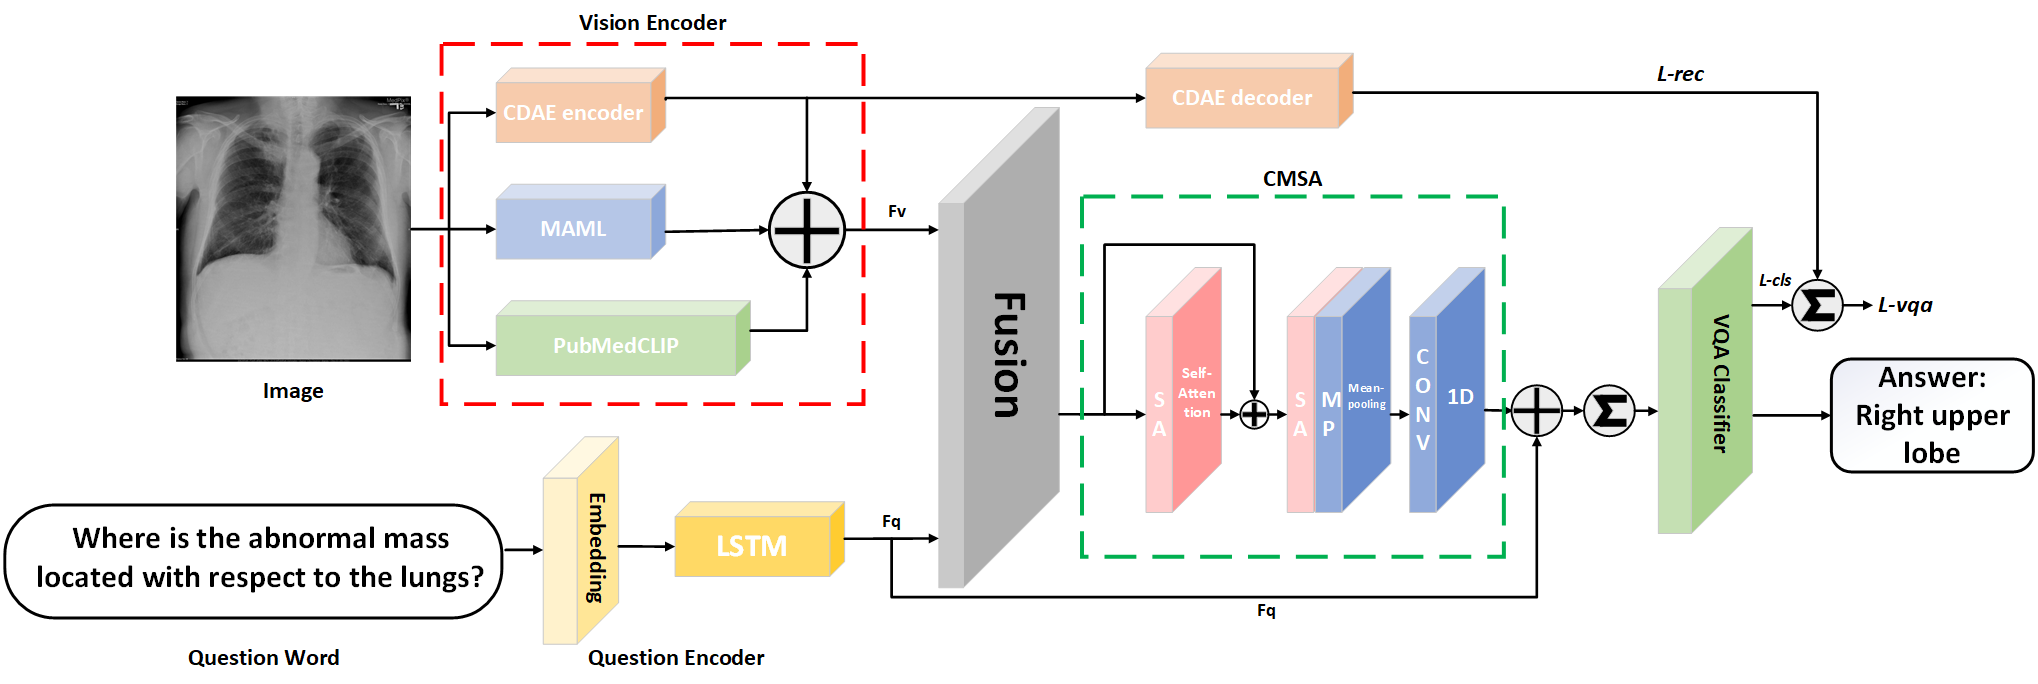
\includegraphics[width=1.1\textwidth]{Fig/myfig/chapter3/modal_net.png}  %scale = 0.3
	% 添加标签one_DFUAV以及图标题“XXX”,引用某图时使用\ref{xxx},其中xxx就是标签,图编号是自动生成的。
	\caption{\label{fig:memsa}多编码融合自注意力网络} 
\end{figure}

MEMSA网络的输入为图像和针对图像提出的开放式或者封闭式文本问题。首先,MEMSA在特征提取部分,使用多个编码器分别提取图像的
特征表示,再使用如图GloVe词编码空间和LSTM网络提取问题的文本特征表示。

接着,在多模态融合部分,先将图像的特征表示和文本的特征表示拼接,拼接后和自身的转置组合成类似于共现矩阵的形式,再对该矩阵计算跨模态自注意力,通过注意力加权
提取出其融合表征,通过残差连接将不同层提取到的信息保持,最终通过每一层特征加和的方式得到一个具有高度相关性的图像-文本联合表征。

最后,在答案推理预测部分,由于Med-VQA的特殊性,将答案预测视为多标签分类问题,使用多层感知机对该联合表征进行求解得到最终的预测,然后再通过
最小化预测与标签之间的交叉熵损失来训练调整模型。接下来各小节将逐一介绍MEMSA各模块的组成和工作原理。

\subsection{各编码器原理}
多编码器的混合的提出最早是为了解决现有医学图像样本的几大缺陷\cite{lin2021medical}:1.样本数量少;2.噪声大,有用信息占比少;3.专业性强,成本高
4.同类图像整体相似度高,难以区分;5.多为灰度图,有用的特征较少。MEMSA网络分别采用降噪自编码器、元学习模型、对比学习预训练模型作为图像编码器。
降噪自编码器可以降低图像噪声,提取有用信息。元学习模型通过在元学习环境中训练的一个通用模型,从而达到在小样本条件下快速适应新任务的效果,十分
适用于医学视觉问答这一领域。对比学习预训练模型由于在大样本预训练时充分学习了图像和语义的对齐关系,所以在编码上有着更丰富的表示,有利于完成开放式问题的回答。
\subsubsection*{图像编码器}
用于MEMSA的图像编码器,由卷积降噪自编码器CDAE、模型不可知元学习模型MAML以及医学对比学习预训练模型PubMedCLIP三个部分混合构成:
\begin{enumerate}[topsep = 0 pt, itemsep= 0 pt, parsep=0pt, partopsep=0pt, leftmargin=44pt, itemindent=0pt, labelsep=6pt, label=(\arabic*)]
	\item 卷积降噪自编码器CDAE
	
	卷积降噪自编码器(Convolutional Denoising Auto-Encoder,CDAE)有编码器和解码器两部分,编码器通过卷积和池化操作提取特征并输出给具有较低维度的隐藏层学习其表示,该表示包含了图像的主要特征而过滤掉了噪声(采用均方误差MSE),再由解码器重新进行上采样重建后获得了更纯净的图像表示,
	DAE首先将原始图像输入$x$(带噪声)映射到保留有用信息的潜在表示$z$,然后再通过解码器将$z$转换为输出$y$。自编码器的训练目标是最小化输出$y$与原始图像$x$之间的重建损失:
	\begin{equation}
		\label{}
		L_{r e c}=\|x-y\|_2^2	
	\end{equation}
	遵循上述原理设计降噪自编码器。为了得到较好的隐变量表示,降噪自编码器由5层卷积层堆栈而成。解码器是一个反卷积层和卷积层的堆栈。带噪声的$x^{\prime}$是通过在原始图像$x$上添加高斯噪声来实现的。
	训练结束后使用编码器和解码器的权值在模型中进行微调。

	\item 模型不可知元学习编码器MAML
	
	基于元学习方法搭建的启发式元学习(Model-Agnostic Meta-Learning,MAML)编码器,其原理为抽取一定数量的样本,在元环境下进行训练得到一个初始化的权重,该权重可以在小样本下就能促进模型达到一个比较好的效果。MAML由带初始化元参数$\theta$的参数化函数$f_\theta$表示。当需要学习一个新任务$T_i$时,设模型参数为$\theta_i^{\prime}$,设训练所用的数据集为$\mathcal{D}$
	样本大小为$N$,在使用元学习方法进行少样本学习时,任务往往可以定义为是一个“k-shot n-way”分类问题。对每个元任务所用的训练集$\mathcal{D^{\prime}}$来源于数据集$\mathcal{D}$
	中的$n$个不同的类,训练时,将$\mathcal{D^{\prime}}$平均分成训练集$\mathcal{D^{tr}}$和验证集$\mathcal{D^{val}}$,每个类包含k个训练图像。迭代h次,生成用于元学习训练批处理的
	$m$个任务,对于每个任务$\mathcal{T}_i$,计算和更新初始化权重的方法如下:
	\begin{equation}
		\label{}
		\theta_i^{\prime}=\theta-\alpha \nabla_\theta L_{\mathcal{T}_i}\left(f_\theta\left(\mathcal{D}_i^{t r}\right)\right)
	\end{equation}
	其中$L_{\mathcal{T}_i}$为任务i的分类损失,在计算完$m$个任务的参数后,通过随机梯度下降(SGD)法更新元模型的参数$\theta$,如下:
	\begin{equation}
		\label{}
		\theta \leftarrow \theta-\beta \nabla_\theta \sum_{\mathcal{T}_i} L_{\mathcal{T}_i}\left(f_{\theta_i^{\prime}}\left(\mathcal{D}_i^{v a l}\right)\right)
	\end{equation}
	遵循上述规则设计元学习编码器。由4层3×3的卷积层,每层卷积后跟着一层归一化层,步幅为2,每个卷积层后接大小为64的BN层进行批次归一化处理,以Relu作为激活函数,解决深度网络中数值不稳定的问题,
	缓解梯度的消失,提高训练效率。

	\item 对比学习预训练编码模型PubMedCLIP
	
	PubMedCLIP是基于PubMed文章数据库对经典CLIP模型进行预训练以及微调得到一个具有医学图像-文本表示能力的编码模型,同时也是一个跨模态模型。PubMedCLIP由图像编码器和文本编码器构成,图像编码器可选用基于CNN的模型,也可以选用基于Transformer的模型;文本编码器可选中基于RNN的模型,同样也可以选用基于Transformer的模型。
	以本文使用到的编码器为例,受制于医学图像的样本数量,选用了样本需求较少的Resnet50模型,然后基于Pelka等人提出的ROCO数据集上对模型进行预训练。对比学习预训练过程是通过计算图像文本对$I-T$之间的
	余弦相似度得到。余弦相似度越大,表明图像$I$和文本$T$的对应关系就越强,反之越弱。所以只需要最大化正样本的余弦相似度,最小化负样本的余弦相似度即可完成优化目标:
	\begin{equation}
		\label{}
		L_{clp}=\min \left(\sum_{i=1}^N \sum_{j=1}^N\left(I_i \cdot T_j\right)_{(i \neq j)}-\sum_{i=1}^N\left(I_i \cdot T_i\right)\right)
	\end{equation}
	其中,N为图像文本样本对$I-T$的个数,训练完成后得到PubMedCLIP的图像编码模型在编码图像时就有了和对应文本的相似关系,从而使得该向量包含了相关含义的语义表示,便于进行下游图像-文本任务以及迁移学习。
\end{enumerate}

\subsubsection*{文本编码器}
用于MEMSA的问题文本编码器,主要分为Word embedding和Question embedding两部分,一个输入文本或者词汇先由Word embedding按照某一词向量空间表示方法将其映射到一个向量表示空间中,成为一个词向量,然后这些词向量再通过Question embedding进行
不同向量间的语义关系建模和学习。
\begin{enumerate}[topsep = 0 pt, itemsep= 0 pt, parsep=0pt, partopsep=0pt, leftmargin=44pt, itemindent=0pt, labelsep=6pt, label=(\arabic*)]
	\item Word embedding
	
	词编码器(Word embedding)是一个词嵌入算法模型,通常由两层全连接神经网络构成,用于学习文本的词向量表示。MEMSA使用GloVe6b作为词向量编码模型,假设有一个大小为V的词汇表,其中包含单词i。GloVe模型中的目标是学习每个单词的向量表示,使得这些向量可以在预测上下文单词和中心单词时发挥良好的作用。
	具体地,GloVe使用一个共现矩阵X来表示单词之间的共现信息,其中$X_{ij}$表示单词i和j在同一个上下文中出现的次数。然后,GloVe定义了每个单词的两个向量表示:中心单词的向量表示$w_i$和上下文单词的向量表示$w_j$。GloVe模型的学习目标是最小化损失函数$J$\eqref{glovegoal}。
	\begin{equation}
		\label{glovegoal}
		J = \frac{1}{2} \sum_{i,j=1}^{|V|} f(X_{ij})(\mathbf{v}_i^T\mathbf{u}j + b_i + b_j - \log X{ij})^2
	\end{equation}
	其中,$f(X_{ij})$是一个权重函数,用于对共现矩阵进行加权。$b_i$和$\tilde{b}_j$是偏置项,用于偏移单词向量表示的值。通过最小化上述损失函数,可以学习到每个单词的向量表示。这些向量表示可以作为文本特征进行使用。
	经医学图像文本预训练的glove词嵌入表示经过t-SNE方法降维后如图\ref{fig:Glove},可知经过一万次的迭代降维后,Glove词向量之间已经在二维平面上初步呈现出各类词向量编码之间的区别,表示数字的语义和具有相似意义的词向量已经被模型
	归类出来划分到了一个具有近似意义的空间中。
	\begin{figure}[htbp]
		% 图片居中(列居中对齐)
		\centering	
		% 包含当前路径下的Fig文件夹的图片文件
		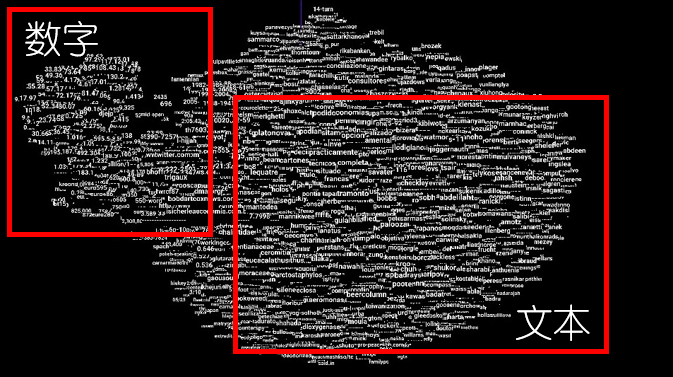
\includegraphics[width=0.8\textwidth]{Fig/myfig/chapter3/glove.png}  %scale = 0.3
		% 添加标签one_DFUAV以及图标题“XXX”,引用某图时使用\ref{xxx},其中xxx就是标签,图编号是自动生成的。
		\caption{\label{fig:Glove}Glove词嵌入的降维表示} 
	\end{figure}
	\item Question embedding
	
	句编码器(Question embedding)是一个用于学习词向量间的语义关系的编码模型,通常可以是循环神经网络(RNN)或者是纯注意力结构。由于医学文本的数据限制,且为了更好地捕获问句序列上下文间的语义联系,MEMSA采用长短时记忆网络\cite{Long short-term memory}(LSTM)作为Quesion embedding。
	如图\ref{fig:lstm},LSTM的基本单元包括三个门(输入门、遗忘门、输出门)和一个记忆细胞,其中输入门控制输入信息的重要性,遗忘门控制上一时刻记忆细胞的重要性,输出门控制输出信息的重要性。记忆细胞可以存储和读取信息,从而实现长期依赖关系的建立和维护。
	\begin{figure}[htbp]
		% 图片居中(列居中对齐)
		\centering	
		% 包含当前路径下的Fig文件夹的图片文件
		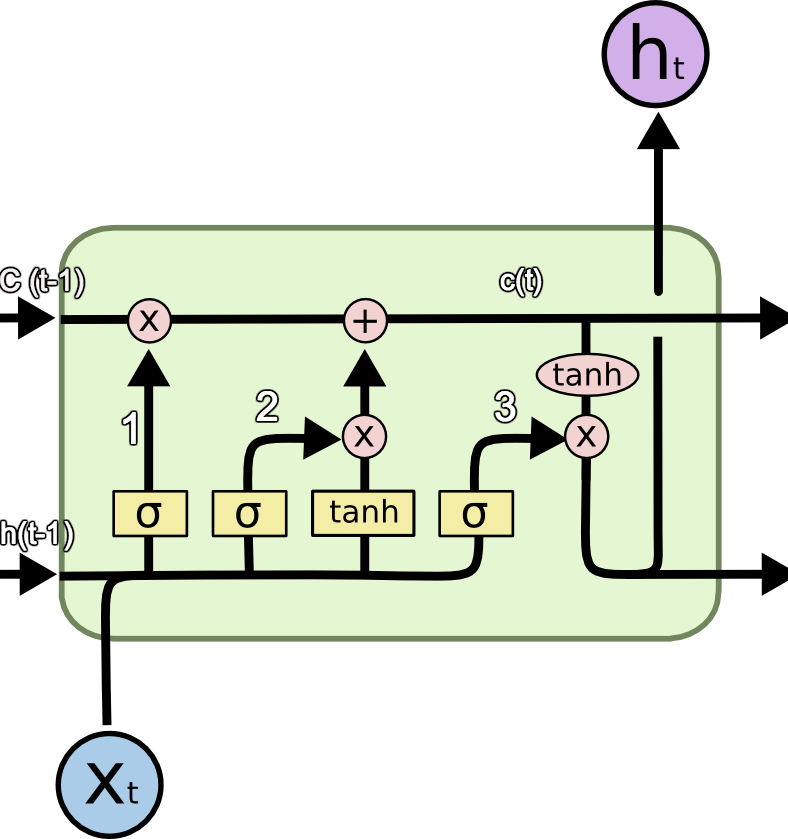
\includegraphics[width=0.5\textwidth]{Fig/myfig/chapter3/lstm.png}  %scale = 0.3
		% 添加标签one_DFUAV以及图标题“XXX”,引用某图时使用\ref{xxx},其中xxx就是标签,图编号是自动生成的。
		\caption{\label{fig:lstm}LSTM网络结构} 
	\end{figure}
	例如在抽取一个句子X的语义特征时,可以使用LSTM来处理这个句子。假设这个句子X包含n个词,每个词用一个d维的词向量表示,那么可以将这个句子的词向量表示为一个n×d的矩阵X=[x1,x2,...,xn],其中xi表示第i个词的d维词向量。
	将这个矩阵输入到LSTM中,经过多个时间步的计算,LSTM会输出一个长度为h的向量表示句子的语义特征,其中h是LSTM的隐藏单元数。这个向量可以作为句子的表示,用于后续的任务,比如分类、聚类等。
\end{enumerate}

\subsection{跨模态自注意力机制}
跨模态自注意力机制由最早P Gao等人\cite{gao2019dynamic}提出,是一种基于自注意力机制实现的跨模态序列融合方法,受Haifan Gong等人\cite{gong2021cross}将其作用在医学图像和文本上的启发。
由于自注意力机制可以通过对序列中不同位置的元素之间的相互作用进行建模来捕捉序列中的长程依赖关系。

如图不同于传统计算图像文本相似度关系的跨模态注意力机制,MEMSA采用的是从图形文本拼接特征中用自注意力机制提取融合特征;不在各模态中单独计算注意力权重矩阵,而是将不同模态特征统一到一个特征空间里进行表示,通过上建立自我内部序列之间的关联来对各模态之间的特征相关关系进行建模,从而捕获更好的图像-语义关联。
本文使用跨模态自注意力机制进行特征融合时,通过先将问题句子按词汇进行词向量拆分,每个词向量再和图像特征进行拼接,最后重新组合成句子。通过这种方式来捕获语义的基本单元-词汇级的细粒度,不但可以把握词汇之间的上下文联系,同时也能把握图像和词汇、文本之间的语义对齐关系。
\begin{figure}[htbp]
	% 图片居中(列居中对齐)
	\centering	
	% 包含当前路径下的Fig文件夹的图片文件
	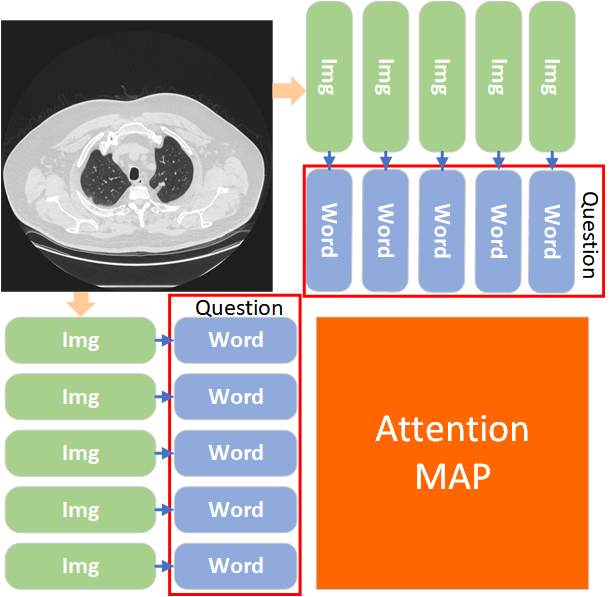
\includegraphics[width=0.6\textwidth]{Fig/myfig/chapter3/attention_map.png}  %scale = 0.3
	% 添加标签one_DFUAV以及图标题“XXX”,引用某图时使用\ref{xxx},其中xxx就是标签,图编号是自动生成的。
	\caption{\label{attention_map}词汇级细粒度融合特征关注图} 
\end{figure}

根据自注意力机制和数学原理,在模态融合前,首先需要将编码得到的视觉特征$v$和问题特征$q$相连接,为了提高表征的细粒度,先将问题特征$q$按词重新拆分,都将其与视觉特征$v$相拼接得到局部特征图$f$,然后重新
合并组合成融合的多模态特征图$F$。然后对该特征图建立注意力矩阵$Q,K,V$,使用3D卷积分别进一步提取$Q,K,V$特征并重塑成二维的特征表示。用该二维特征与其自身的转置相乘得到特征之间的关联表示,再经过softmax函数缩后放后就得到了对应
的注意力图:
\begin{equation}
	\label{}
	A = softmax(QK^{T})
\end{equation}
这样,注意力图A中就蕴含了融合特征$F$内各部分特征之间的相关关系,相比于一维序列上的自注意力,这是一种在二维特征图上的自注意力机制。接着,特征图$V$经过注意力$A$加权后得到注意力增强的多模态表示$F^{\prime}$:
\begin{equation}
	\label{}
	F^{\prime} = A V
\end{equation}
经过注意力增强后$F^{\prime}$再次经过转置,重塑,反卷积操作还原成最初多模态特征图$F$的形状,此外,受到Resnet网络结构的启发,多次重复了注意力模块并使用残差连接保留所有的局部特征。经过均值和池化处理后,
最终的多模态表示为:
\begin{equation}
	\label{}
	\hat{F}_i=\frac{\sum_{j=1}^m \sum_{k=1}^n\left(F_{i j k}^{\prime}+F_{i j k}\right)}{m \times n}
\end{equation}
其中$i,j,k$为特征图$F$构建时所包含的词汇数位以及特征图高度、宽度,$m,n$为该特征图总尺寸,最终$\hat{F}_i$经过线性层映射到和文本特征$q$相同的维度。

\section{模型预测与网络训练}
\subsection{模型预测}
感知机(Multilayer Perceptron,MLP)是一种简单、常用的分类网络,有输入层,隐藏层,输出层组成,并且各层皆为全连接网络。输入层接收数据,隐藏层对数据进行非线性变换和特征提取,提高数据的表达能力,层数越多,
感知机对特征的抽象能力往往越强,内部非线性由激活函数激活,最后计算输出损失,根据反向传播算法优化网络的权重和偏置,从而达到学习的效果。医学视觉问答由于分为开放式问答
和封闭式问答,对于检索式问答系统,可将这两种问答分别看成是多标签分类问题和二分类问题。为了提高模型的简洁度,MEMSA模型同样将yes,no同样视为两个独立的标签参与多分类
虽然给分类增加了难度,但也打开了问题形式的局限。多标签分类问题往往通过计算多标签损失(MSE)来作为梯度信息进行反向传播。
多模态表示$\hat{F}$经过线性映射后维度和问题$q$相同,与问题$q$句子中的所有词上进行求和,最后将其输入到一个两层MLP中进行答案预测,获得答案的预测分数$s$,答案的预测分数计算如表达式\eqref{mlp_preds}:
\begin{equation}
	\label{mlp_preds}
	s=M L P\left(\sum_{i=1}^{N}\left(\hat{F}_i+q_i\right)\right) 
\end{equation}
变量$N$为控制问题句子长度的超参数,同时也指示问题句子所包含的词汇个数。

\subsection{网络训练}
MEMSA模型由多个部分组成,包括图像编码,问题编码,跨模态注意力融合以及答案预测。故采用多任务损失并以端到端的方式训练模型:
\begin{equation}
	\label{}
	L=L_{vqa}+\alpha L_{rec} 
\end{equation}
$L_{vqa}$是基于分类的答案预测和标签之间的交叉熵损失;$L_{rec}$如上述是自编码器输出$y$与原始图像$x$之间的重建交叉熵损失。$\alpha$是平衡两个
损失项的超参数,往往设置为0.5。
\subsubsection*{实验超参数设置}
模型的超参数设定如表\ref{tab:su_para}:
\begin{table}
	\centering
	\caption{\label{tab:su_para}模型超参数设置}
	\small
	\begin{tabular}{ccccc}
		\hline
		参数名 & 参数值 & 参数含义 \\
		\hline Word token & 12 & 输入问句的划分长度 \\
		Word embedding dim & 600 & 词向量维度(GloVe) \\
		Visual feature dim & 1152 & 图像特征维度 \\
		LSTM dim & 1024 & 文本特征维度 \\
		Joint feature dim1 & 2184 & 多编码特征混合后的的维度 \\
		Joint feature dim2 & 1024 & 特征经注意力融合后的的维度 \\
		Batch Size & 32 & 训练批量大小 \\
		Learn rate & (0,0.01) & 动态学习率区间 \\
		\hline
	\end{tabular}
\end{table}


% \subsubsection{网络参数}
% 如图\ref{fig:cmae},图像在经过降噪自编码器、元学习模型、对比学习预训练模型后会得到3个特征分量,3个分量经过一定的维度处理后融合成图像特征向量fv。
% 同时,文字经过词嵌入转换以及编码后得到了文本特征向量fq。两大模态的特征向量经过Fusion处理后输入到跨模态自注意力模块。
% 模块用于捕获模态间联系,然后将处理后的融合特征向量交由分类器模型得到最终的预测。预测和真值之间计算多标签交叉熵损失Lcls。
% 值得一提的是,为了提高降噪自编码器的性能,模型还引入了损失Lrec,最终的损失由二者求和得到。模型属性和参数如下表所示:
% \begin{table}
% 	\caption{\label{tab:modal_para}模型结构以及相应参数}
% 	\centering
% 	\small
% 	\begin{tabular}{ccc}
% 		\hline
% 		模型结构 & 网络层数 & 参数量 \tabularnewline
% 		\hline
% 		DAE & $5Conv2d$ & $1283745$ \tabularnewline
% 		MAML & $2$ & $1283745$ \tabularnewline
% 		CLUP & $2$ & $1283745$ \tabularnewline
% 		WEMB & $2$ & $353400 * 2$ \tabularnewline
% 		QEMB & $2$ & $2457600$ \tabularnewline
% 		CMSA & $2$ & $2384928$ \tabularnewline
% 		MLP & $2$ & $1283745$ \tabularnewline
% 		ALL & $2$ & $138003102$ \tabularnewline
% 		\hline
% 		% \midrule
% 		% 数据集 & Images & QApairs \\
% 		% VQA2.0 & 204k &  614K\\
% 		% VQA-Med-2018 & 1 & 3.00 \\
% 		% \bottomrule
% 	\end{tabular}
% \end{table}
\subsubsection*{实验条件与环境}
实验环境设置如表\ref{tab:env_para}:
\begin{table}
	\caption{\label{tab:env_para}深度学习环境配置}
	\centering
	\small
	\begin{tabular}{cc}
		\hline 环境名称 & 版本 \\
		\hline 处理器 & Intel(R) Xeon(R) CPU E5-2620 v4 @ 2.10GHz \\
		内存 & $64 \mathrm{~GB}$ \\
		操作系统 & Ubuntu 18.04 \\
		开发语言 & Python 3.6 \\
		GPU & NVIDIA TITAN Xp 12GB \\
		CUDA & CUDA Toolkit 11.2 \\
		深度学习开发库 & Pytorch 1.7.1 for GPU \\
		\hline
		\end{tabular}
\end{table}

\section{实验结果}
\subsection{编码器模型实验对比分析}
目前各混合视觉增强方法在Med-RAD、SLAKE数据集上的开放式问答,封闭式问答,以及总准确率如表\ref{tab:modal_red_cmp}。其中,因为SLAKE数据集缺少MTPT方法所需要的图像来源标签,所以此处不予计算和讨论。
\begin{table}
	\caption{\label{tab:modal_red_cmp1}MEMSA与主流方法等对比}
	\centering
	\small
	\begin{tabular}{l|lll|lll}
		\hline Dataset & \multicolumn{3}{l}{\textbf{Med-RAD}} & \multicolumn{3}{|l}{\textbf{SLAKE}} \\ 
		\hline Methods & Open & Closed & ALL & Open & Closed & ALL\\
		\hline RAD-SAN\cite{lau2018dataset} & $24.2 \%$ & $57.2 \%$ & $44.0 \%$ & X & X & X\\
		RAD-MCB\cite{lau2018dataset} & $25.4 \%$ & $60.6 \%$ & $46.5 \%$ & X & X & X\\
		\hline MVEF-BAN \cite{nguyen2019overcoming} & $43.9 \%$ & $75.1 \%$ & $62.7 \%$ & $75.0 \%$ & $76.4 \%$ & $75.6 \%$ \\
		MTPT-BAN & $47.2 \%$ & $77.8 \%$ & $65.6 \%$ & X & X & X\\
		CPAE-BAN\cite{eslami2021does} & $48.6 \%$ & $78.1 \%$ & $66.5 \%$ & $76.2 \%$ & $79.9 \%$ & $77.6 \%$\\
		MEMBA & $52.0 \%$ & $78.0 \%$ & $68.3 \%$ & $76.3 \%$ & $78.6 \%$ & $77.2 \%$\\
		\hline MVEF-CMSA & $43.9 \%$ & $75.1 \%$ & $62.6 \%$ & $75.8 \%$ & $81.5 \%$ & $78.0 \%$\\
		MTPT-CMSA\cite{gong2021cross} & $56.1 \%$ & $77.3 \%$ & $68.8 \%$ & X & X & X\\
		CPAE-CMSA & $63.7 \%$ & $76.1 \%$ & $71.2 \%$ & $77.2 \%$ & $81.5 \%$ & $78.9 \%$\\
		MEMSA & $\mathbf{65.4 \%}$ & $\mathbf{77.6 \%}$ & $\mathbf{72.7 \%}$ & $76.0 \%$ & $\mathbf{81.7 \%}$ & $78.2 \%$\\
		\hline
		\end{tabular}
\end{table}

从表\ref{tab:modal_red_cmp1}可以预见,在使用经典的双线性池化注意力机制(BAN)以及跨模态自注意力机制(CMSA)作为融合网络时,PubMedCLIP的使用和在多编码器混合作用的效果下,模型在小样本数据集Mad-RAD下的开放式
问答表现有着明显的提高,采用多编码器混合加双线性池化注意力机制MEMBA这一方法,相比18年Binh等人提出的基线模型MVEF-BAN\cite{nguyen2019overcoming},MEMBA模型针对开放式回答的效果提升了8.1\%,封闭式回答提升了2.9\%,总体性能提升了5.6\%。
采用MEMSA模型,综合性能分别提升了21.5\%、2.5\%和10\%。在SLAKE数据集上,MEMBA综合提升了1\%~2\%,MEMSA提升了2\%~3\%,性能提升不明显的主要原因是SLAKE数据量级较大,模型抽取的特征相对完备,
单一或简单编码器组合也能取得良好的性能,就会会导致针对小样本情况下设计的MEMSA带来的性能提升不明显。综上,通过采用具有不同功能的多编码器混合以及跨模态自注意力方法,MEMSA可以通过提升特征的多样化表示,在开放式问题下获得更好的性能效果,
从而提升模型整体的问答性能。
% \subsection{消融实验:使用不同编码器对比分析}
% 基于同一融合注意力模型,使用不同编码器时,模型取得的性能如下表:
% \begin{enumerate}[topsep = 0 pt, itemsep= 0 pt, parsep=0pt, partopsep=0pt, leftmargin=44pt, itemindent=0pt, labelsep=6pt, label=(\arabic*)]
% 	\item:各模型在Med-RAD数据集上的开放式问答,封闭式问答,以及总准确率。
	
% 	\item 各模型在SLAKE数据集上的开放式问答,封闭式问答,以及总准确率。
	
% \end{enumerate}

\subsection{注意力模型实验对比分析}
\begin{table}
	\caption{\label{tab:modal_red_cmp2}不同注意力下的模型性能对比}
	\centering
	\small
	\begin{tabular}{l|lll|lll}
		\hline Dataset & \multicolumn{3}{l}{\textbf{Med-RAD}} & \multicolumn{3}{|l}{\textbf{SLAKE}} \\ 
		\hline Methods & Open & Closed & ALL & Open & Closed & ALL\\
		\hline MVEF-SAN\cite{nguyen2019overcoming} & $40.7 \%$ & $74.1 \%$ & $60.8 \%$ & $72.9 \&$ & $77.6 \%$ & $74.7 \%$\\
		MVEF-BAN\cite{nguyen2019overcoming} & $43.9 \%$ & $75.1 \%$ & $62.6 \%$ & $75.0 \%$ & $76.4 \%$ & $75.6 \%$\\
		MVEF-CMSA & $43.9 \%$ & $75.1 \%$ & $62.6 \%$ & $75.8 \%$ & $81.5\%$ & $78.0\%$\\
		\hline MTPT-SAN & $43.0 \%$ & $72.8 \%$ & $61.0 \%$ & X & X & X\\
		MTPT-BAN\cite{gong2021cross} & $56.1 \%$ & $75.7 \%$ & $67.9 \%$ & X & X & X\\
		MTPT-CMSA\cite{gong2021cross} & $56.1 \%$ & $77.3 \%$ & $68.8 \%$ & X & X & X\\
		\hline MEM-SAN & $53.6 \%$ & $75.7 \%$ & $67.0 \%$ & $74.9 \%$ & $82.0 \%$ & $77.7 \%$\\
		MEM-BAN & $52.0 \%$ & $78.0 \%$ & $68.3 \%$ & $\mathbf{76.3} \%$ & $78.6 \%$ & $77.2 \%$\\
		MEMSA & $\mathbf{65.4 \%}$ & $77.6 \%$ & $\mathbf{72.7 \%}$ & $76.0 \%$ & $81.7 \%$ & $\mathbf{78.2 \%}$\\
		\hline
		\end{tabular}
\end{table}
使用不同注意力机制时,模型性能如表\ref{tab:modal_red_cmp2}。固定同一编码方式为MVEF、MTPT、MEM的情况下,采用几个常用的基于注意力的特征融合方法:
堆叠注意力机制(SAN),双线性池化注意力机制(BAN)和跨模态自注意力(CMSA)进行对比分析:在Med-RAD数据集上,每种注意力之间呈现逐渐递增的态势。
并且发现编码器多样性越高,跨模态自注意力机制的效果就越明显,这充分说明了自注意力在跨模态或者多模态信息的建模上具有独特的优势。

并且通过三类编码方案综合对比,多编码器混合方式对于各种注意力融合机制具有最佳的适配性,在SAN、BAN等传统方法上都可以大幅度提升性能。
在数据量较大,基准准确率较高的SLAKE数据集上,模型的综合性能也得到了小幅度提升。

\subsection{实验总结}
综合上述实验,在使用不同的编码方式时,具有不同作用的多编码器可以提高模型的表征能力,提高模型的分类准确率;

我们知道,向量之间的主要运算有cat,sum,mul等形式。受空间约束和相关性的影响,属于不同模态,代表不同意义的向量之间无法直接产生有效的运算形式。
如果不经过坐标变换,映射,归一化等操作再运算的话则会导致严重的信息丢失。可以预见,在神经网络中,直接拼接组合是相比于运算更为有利的信息融合方式。
因为维度代表一种信息的尺度,在编码时,每增加一个维度就会带来这个信息新的“描述”,从而提升了这个信息的表达能力和空间上的可区分度。
值得注意的是,不同的编码器在编码同一信息时难免会产生冗余,比如描述的向量空间中的某些分量是呈现线性相关的。这时侯就会引入重复的信息和增大特征维度
给模型设计和计算资源带来难题。

而且相比于传统的特征处理方式,基于注意力是一种更为灵活,高效,而且可以由神经网络自发的学习和选择不同模态中的有效特征的一种
多模态融合方式。为了解决不同模态编码信息维度之间有效匹配的问题本文采取了词汇级细粒度表征的跨模态自注意力的方法,
跨模态自注意力通过计算不同模态信息之间的匹配程度得到这些信息维度的重要性权值用于筛选出真正有效(线性无关)的特征信息,
从而实现更高效地捕获不同模态间的联系以及和自身的上下文关联。

\section{讨论}
为了更加深入地了解多模态混合自注意力网络的机制,理解其提升医学视觉问答效果的途径和原理,本小节将继续讨论MEMSA网络具体回答Med-RAD数据集中某一类问题的能力,同时对MEMSA网络的分类预测
能力进行综合评估,最后通过问答样例对比直观地感受MEMSA网络在回答医学视觉问题时的实际效果。
\subsection{按问题类型划分的准确率比较}
除上述表\ref{tab:modal_red_cmp1,tab:modal_red_cmp2}中针对回答方式(OPEN,CLOSE)的划分外,还可以针对不同的提问内容(如提问计数、颜色、尺寸、模态等)进行问答划分,分析
Med-VQA模型在不同内容提问下的准确率。
用Med-RAD数据集进行模型性能测试,其在开放式问答和封闭式问答中针对具体的回答内容的分类性能分别如表\ref{tab:qt-close-end}和表\ref{tab:qt-open-end},
\begin{table}
	\caption{\label{tab:qt-close-end}CLOSE-Question Results}
	\centering
	\small % 调整表格字号
	\begin{tabular}{l|lllll|lllll} %右边补MVEF-BAN的性能
		\hline Model & \multicolumn{5}{l}{\textbf{MEMSA}} & \multicolumn{5}{|l}{\textbf{MVEF-BAN}(base)} \\ 
		\hline QA-type & count & real & TRUE & real \% & score \% & count & real & TRUE & real \% & score \%\\ 
		\hline COUNT & 4 & 4 & 3 & 100 \%& 75 \%& 4 & 4 & 3 & 100 \%& 75 \%\\
		COLOR & 4 & 4 & 4 & 100 \%& 100 \%& 4 & 4 & 4 & 100 \%& 100 \%\\
		ORGAN & 2 & 2 & 2 & 100 \%& 100 \%& 2 & 2 & 2 & 100 \%& 100 \%\\
		PRES & 124 & 124 & 106 & 100 \%& $\mathbf{85.5 \%}$& 124 & 124 & 104 & 100 \%& 83.9 \%\\
		PLANE & 12 & 11 & 7 & 91.7 \%& $\mathbf{58.3 \%}$& 12 & 11 & 4 & 91.7 \%& 33.3 \%\\
		MODALITY & 17 & 17 & 12 & 100 \%& $\mathbf{70.6 \%}$& 17 & 17 & 8 & 100 \%& 47.1 \%\\
		POS & 8 & 8 & 5 & 100 \%& $\mathbf{62.5 \%}$& 8 & 8 & 4 & 100 \%& 50 \%\\
		ABN & 38 & 35 & 28 & 92.1 \%& 73.7 \%& 38 & 35 & 28 & 92.1 \%& 73.7 \%\\
		SIZE & 41 & 40 & 35 & 97.6 \%& 85.4 \%& 41 & 40 & 35 & 97.6 \%& 85.4 \%\\
		OTHER & 11 & 10 & 4 & 90.9 \%& 36.4 \%& 11 & 10 & 8 & 90.9 \%& 72.7 \%\\
		ATTRIB & 16 & 16 & 14 & 100 \%& 87.5 \%& 16 & 16 & 15 & 100 \%& 93.8 \%\\
		\hline
		\end{tabular}
\end{table}

\begin{table}
	\caption{\label{tab:qt-open-end}OPEN-Question Results}
	\centering
	\small % 调整表格字号
	\begin{tabular}{l|lllll|lllll}
		\hline Model & \multicolumn{5}{|l}{\textbf{MEMSA}} & \multicolumn{5}{|l}{\textbf{MVEF-BAN}(base)} \\ 
		\hline QA-type & count & real & TRUE & real \% & score \% & count & real & TRUE & real \% & score \%\\
		\hline COUNT & 2 & 2 & 2 & 100 \%& 100 \%& 2 & 2 & 2 & 100 \%& 100\%\\
		COLOR & 0 & 0 & 0 & 0 \%& 0 \%& 0 & 0 & 0 & 0 \%& 0\%\ \\
		ORGAN & 8 & 6 & 3 & 75 \%& 37.5 \% & 8 & 6 & 3 & 75 \%& 37.5\%\\
		PRE & 47 & 36 & 31 & 76.6 \%& $\mathbf{66 \%}$ & 47 & 36 & 21 & 76.6 \%& 44.7\%\\
		PLANE & 14 & 13 & 11 & 92.9 \%& 78.6 \% & 14 & 13 & 11 & 92.9 \%& 78.6\%\\
		MODALITY & 14 & 10 & 3 & 62.5 \%& 18.8 \% & 16 & 10 & 5 & 62.5 \%& 31.2\%\\
		POS & 53 & 47 & 42 & 88.7 \%& $\mathbf{79.2 \%}$& 53 & 47 & 40 & 88.7 \%& 75.5\%\\
		ABN & 18 & 18 & 17 & 100 \%& $\mathbf{94.4 \%}$& 18 & 18 & 11 & 100 \%& 61.1\%\\
		SIZE & 5 & 5 & 3 & 100 \%& 60 \%& 5 & 5 & 4 & 100 \%& 80\%\\
		OTHER & 15 & 3 & 0 & 20 \%& 0 \%& 15 & 3 & 0 & 20 \%& 0\%\\
		ATTRIB &4 &4 &3 & 100 \%& 75 \%& 4 & 4 & 3 & 100 \%& 75 \% \\
		\hline
		\end{tabular}
\end{table}

可见,MEMSA模型的性能提升主要来自于其能够更好回答开放式问答和封闭式问答中有关PRES、PLANE、MODALITY、POS这几类数据集占比较大的问题。
\subsection{MEMSA模型综合评估}
建立模型预测的混淆矩阵是综合评价一个模型分类性能的有效方法,对于一个分类模型,可以建立一个类别数为N的混淆矩阵,行表示预测标签,列表示真实标签。
矩阵中的每个元素表示真实标签和预测标签的组合,即在真实标签为该行所表示的标签时,模型预测为该列所表示的标签的样本数量。在非生成式视觉问答场景中,
封闭式问答为归为一个二分类问题,开放式问答可以归为一个多分类问题,Li-Ming Zhan等人给模型增加了一个即插即用的QCR和TCR模块\cite{zhan2020medical}用于问题分类,
并解释了将问题按照类型进行事先划分可以更好地提高模型问答的准确率。通过观察混淆矩阵\ref{close_confusionmatrix}和\ref{open_confusionmatrix},
可以直观地了解模型的对各问题的分类情况,例如哪些类别容易被混淆、哪些类别分类效果较好等,进而对模型进行优化。
% \begin{figure}
% 	% 居中
% 	\centering	
% 	% 包含当前路径下的Fig文件夹的图片文件
% 	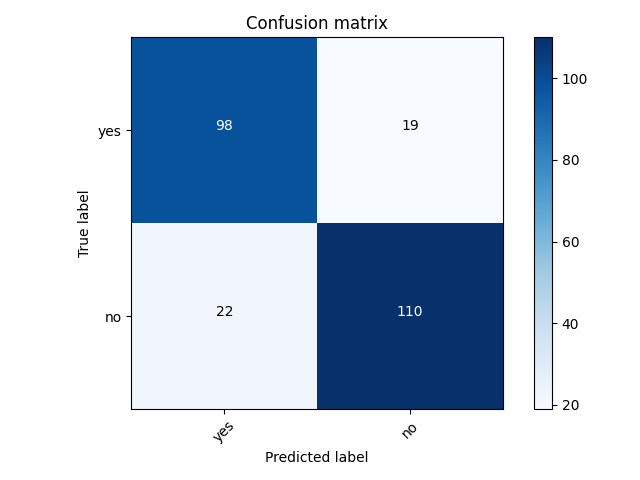
\includegraphics[width=0.8\textwidth]{Fig/myfig/chapter3/close_confusionmatrix.png}  %scale = 0.3
% 	% 添加标签one_DFUAV以及图标题“XXX”,引用某图时使用\ref{xxx},其中xxx就是标签,图编号是自动生成的。
% 	\caption{\label{close_confusionmatrix}MEMSA封闭式问答混淆矩阵} 	
% \end{figure}

% \begin{figure}
% 	% 居中
% 	\centering	
% 	% 包含当前路径下的Fig文件夹的图片文件
% 	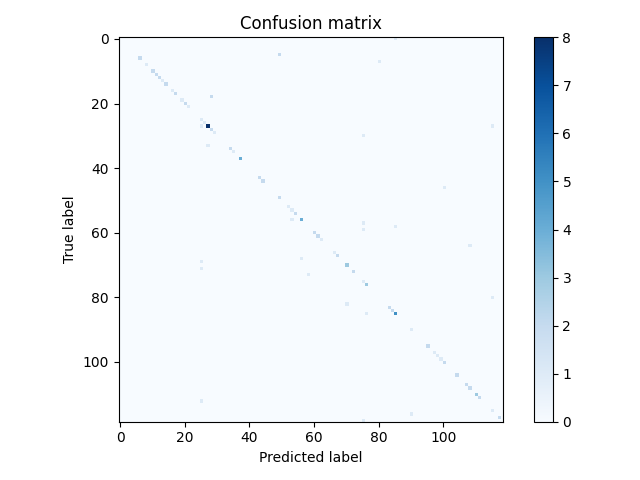
\includegraphics[width=0.8\textwidth]{Fig/myfig/chapter3/open_confusionmatrix.png}  %scale = 0.3
% 	% 添加标签one_DFUAV以及图标题“XXX”,引用某图时使用\ref{xxx},其中xxx就是标签,图编号是自动生成的。
% 	\caption{\label{open_confusionmatrix}MEMSA开放式问答混淆矩阵} 	
% \end{figure}

\begin{figure}[htbp]
	\begin{minipage}{0.5\linewidth}
		\centering	
		% 包含当前路径下的Fig文件夹的图片文件
		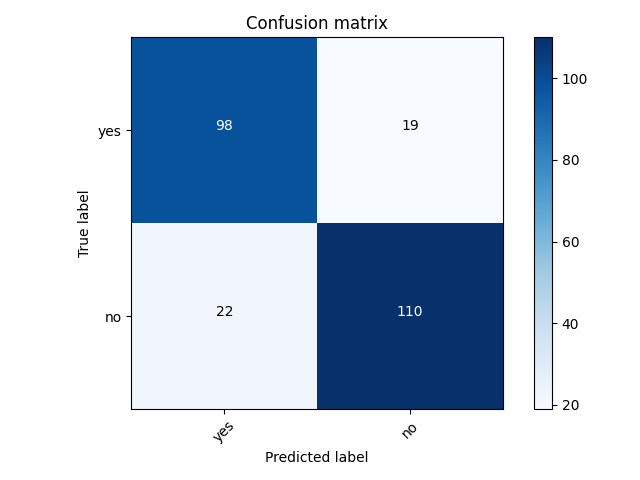
\includegraphics[width=1.1\textwidth]{Fig/myfig/chapter3/close_confusionmatrix.png}  %scale = 0.3
		% 添加标签one_DFUAV以及图标题“XXX”,引用某图时使用\ref{xxx},其中xxx就是标签,图编号是自动生成的。
		\caption{\label{close_confusionmatrix}封闭式问答混淆矩阵} 	
	\end{minipage}
	% 图片居中(列居中对齐)
	\begin{minipage}{0.5\linewidth}
		\centering	
		% 包含当前路径下的Fig文件夹的图片文件
		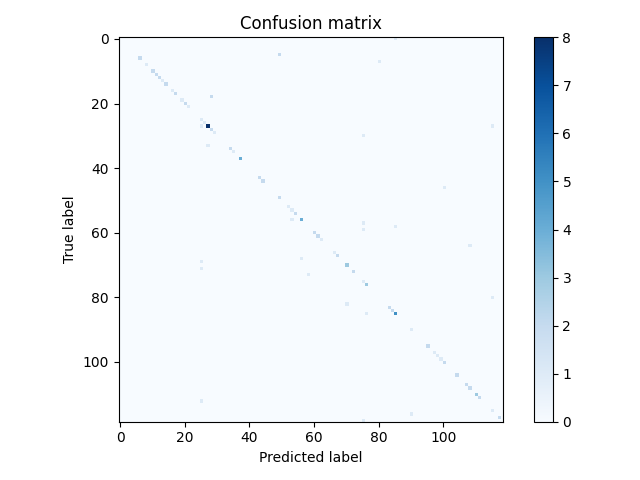
\includegraphics[width=1.1\textwidth]{Fig/myfig/chapter3/open_confusionmatrix.png}  %scale = 0.3
		% 添加标签one_DFUAV以及图标题“XXX”,引用某图时使用\ref{xxx},其中xxx就是标签,图编号是自动生成的。
		\caption{\label{open_confusionmatrix}开放式问答混淆矩阵} 	
	\end{minipage}	
\end{figure}

\begin{table}
	\caption{\label{tab:confusionmatrix}不同方法的综合性能对比}
	\centering
	\small
	\begin{tabular}{c|cccccc}
		\hline  方法 & TP(sum) & TN(sum) & FP(sum) & Precision(avg) & Recall(avg) & F1(avg) \\
		\hline MVEF-BAN & 290 & 73 & 73 & 0.658 & 0.643 & 0.644 \\
		CPAE-BAN & 282 & 72 & 72 & 0.671 & 0.625 & 0.637 \\
		MTPT-CMSA & 296 & 89 & 89 & 0.648 & 0.656 & 0.645 \\
		MEMSA & 309 & 73 & 73 & 0.685 & 0.685 & $\mathbf{0.678}$ \\
		\hline
		\end{tabular}
\end{table}

对于分类检索式问答来说,准确率如表\ref{tab:modal_red_cmp}代表了模型分类到正确的答案占总样本数的比例,它反映了模型整体的分类性能也是最重要的指标;
关于表\ref{tab:confusionmatrix},精确率表示模型在预测为正例的样本中真正为正例的样本数占预测为正例的样本数的比例,它反映了模型在预测为正例的样本中的准确程度,
从表中可得知,MEMSA模型具有最大的Precision值,相较于主流模型具有比较优秀的精度,可以充分保证回答的质量;
召回率是指模型在所有真正的正例样本中预测为正例的样本数占所有真正的正例样本数的比例,它反映了模型在发现真正的正例样本方面的能力。
同样,MEMSA也具有最大的Recall值,在问答时尽可能地预测出所有正确的回答。F1分数是精确率和召回率的调和平均数,它综合了精确率和召回率的优缺点,
用于综合评价模型的性能,综合来看MEMSA具有最高的F1分数,说明MEMSA相较其他主流模型存在优势。
\begin{figure}[htbp]
	% 图片居中(列居中对齐)
	\centering	
	% 包含当前路径下的Fig文件夹的图片文件
	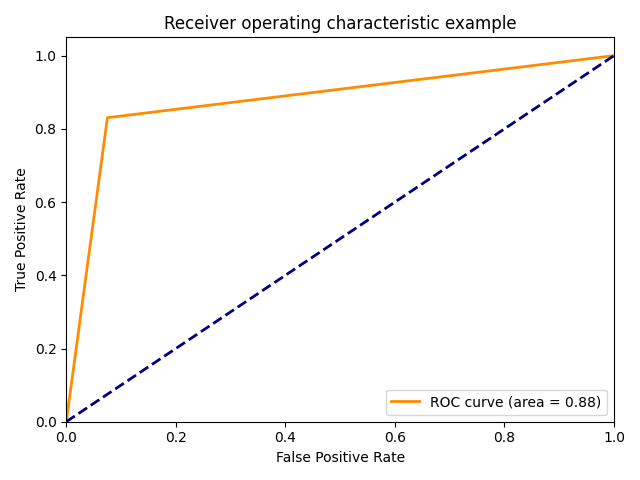
\includegraphics[width=0.8\textwidth]{Fig/myfig/chapter3/all_roc.png}  %scale = 0.3
	% 添加标签one_DFUAV以及图标题“XXX”,引用某图时使用\ref{xxx},其中xxx就是标签,图编号是自动生成的。
	\caption{\label{all_roc}封闭式问答模型ROC曲线} 
\end{figure}

% \subsection{编码器隐变量表征分析}
% 图像在网络中的表征往往用隐变量来表示,分析三个编码器是如何达到降噪、减小样本使用、获得更多表征能力的。

% \subsection{信号扰动实验}
从图\ref{all_roc}可以看出,对于回答封闭式这一二元分类问题,在模型默认的绝对分类阈值以及分类方式下,模型AUC值达到0.88,说明MEMSA模型在回答二分类问题时具有较强的泛化能力。
由于开放式问答(多标签分类问题)的ROC曲线不具有显著的实际意义,故本文在此不做详细讨论。

\subsection{MEMSA实例问答效果}
为了直观地展现MEMSA在医学视觉问答上的实际效果,具体问答样例如图\ref{fig:qa_demo},选用MEMSA和基线模型MEVF-BAN作问答对比,
模型在做开放式问答时,MEMSA准确预测了问题出现在肺叶的右上叶(right upper lobe),相比于采用双线性池化的MVEF-BAN模型预测的不具备直接语义的回答“right upper base”
MEMSA具有更好的细粒度语义解析能力和对语句序列的上下文进行语义建模的能力。同时,在具有多个正确答案的开放式问答图中具有什么器官中,主流模型往往倾向于回答脊髓(spinal cord)
MEM
\begin{figure}[htbp]
	% 图片居中(列居中对齐)
	\centering	
	% 包含当前路径下的Fig文件夹的图片文件
	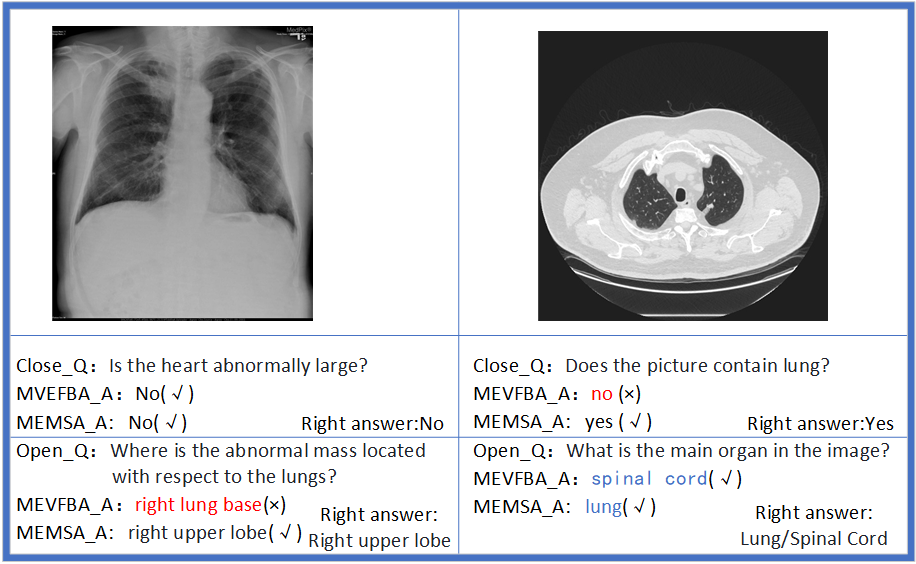
\includegraphics[width=0.8\textwidth]{Fig/myfig/chapter3/qa_demo.png}  %scale = 0.3
	% 添加标签one_DFUAV以及图标题“XXX”,引用某图时使用\ref{xxx},其中xxx就是标签,图编号是自动生成的。
	\caption{\label{fig:qa_demo}MEMSA与MEVFBA(MAML+AE-BAN)的回复比较} 
\end{figure}


\section{本章小结}
本章首先介绍了主流视觉问答网络的实现原理和总体架构,包括特征提取、特征融合和答案预测等组件。接着,根据目前主流模型的一些缺陷
和医学视觉问答的特点,提出了多编码器混合自注意力模型MEMSA。然后在具体的实验部分介绍了使用的数据集和模型细节,实验所处的环境和实验条件。
本章在实验中从整体性能,问答类型性能等多个角度综合对比了多编码器混合自注意力模型相比于主流模型的性能差异并对原因进行了分析,
接着做了分解对照实验,固定编码器模型,重新分析了不同注意力模型对问答性能的影响,证明了多编码器模型在非跨模态自注意力模型的情况下也能提升部分模型性能,
说明了正确使用多模态编码模型时的一个优越性。













